\documentclass[10pt]{article}
\usepackage{icmlko}

\icmlmeta{IP 파운데이션 월드모델}{145}{깊이가 범인이었고, 배깅은 값을 안 받는다}{노트 144가 찾은 전파의 원인을 두 번 틀리게 짚고 세 번째에 맞혔다 --- 틀린 이유가 지표였다}

\begin{document}

\twocolumn[
\icmlheader

\begin{abstract}
노트 144가 남긴 첫 줄은 ``F8은 왜 유독 전파가 큰가''였다. 세 번 짚었다.
\textbf{두 번 틀렸고 틀린 이유가 같다} --- 지표가 잡음이었다. 노트 144의
귀착 바닥은 ``섭동 다섯 판의 $\rho$ 최대$-$최소''인데 팝업 $n=59$에서 그
자체가 흔들린다. 그걸로 재니 깊이 1에서도 0.067이라 ``깊이는 무관''이라
읽었고, 배깅해도 0.063이라 ``탐욕 선택도 아니다''라고 읽었다. \textbf{둘 다
틀렸다.} 지표를 바꾸니 --- 섭동 전후 \emph{예측 순위}의 자기상관, 라벨을
아예 안 보는 값 --- 신호가 단조로 드러난다. \textbf{깊이 1 · 2 · 4에서
0.981 · 0.951 · 0.895다.} 도메인 표시자를 빼도 0.882로 안 변하고(원인이
아니다), 반복을 220에서 800으로 늘려도 소수 셋째까지 같다(수렴했다), 예측이
겹쳐서도 아니다(59개가 전부 다른 값이다). \textbf{원인은 상호작용 깊이다} ---
깊게 쓸수록 풀이 조금 바뀔 때 함수가 통째로 다시 짜인다. 그러면 깊이를
낮추면 되는데 판이 $+$0.366에서 $+$0.338로 내린다. \textbf{배깅은 둘 다
산다} --- 부트스트랩 여덟 개의 순위 평균이 자기상관 0.951에 판 $+$0.3846으로
현행($0.895$ · $+0.3661$)을 두 축 모두에서 이긴다. \textbf{그런데 챔피언
설정에서는 점수가 안 온다.} 문턱 15에서 판 $\rho$가 F8 $+$0.4409 대 배깅
$+$0.4396으로 사실상 같다. 그래서 채택 근거는 점수가 아니다 --- \textbf{같은
점수에 흔들림 절반}(0.906 → 0.948)이다. 노트 133의 규칙대로, 한 설정에서
나온 $+$0.0185는 채택 사유가 아니다.
\end{abstract}
]

\begin{figure*}[t]
\centering
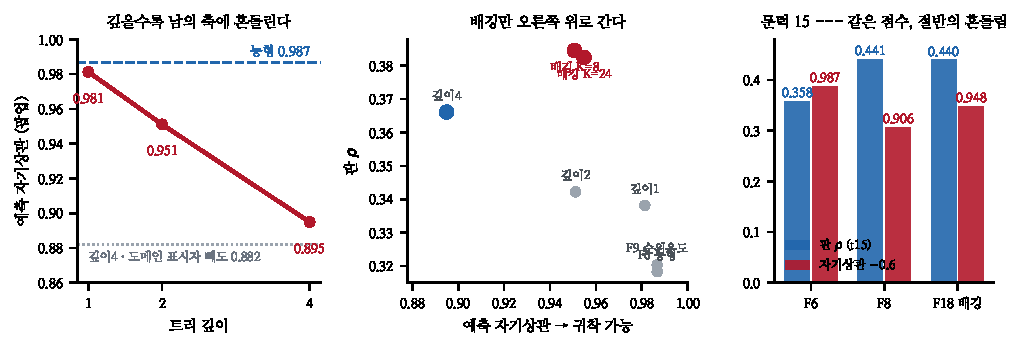
\includegraphics[width=\textwidth]{figs/stab.pdf}
\caption{왼쪽 --- 깊이가 원인이다. 가운데 --- 배깅만 오른쪽 위로 간다.
오른쪽 --- 챔피언 설정에서는 점수가 같고 흔들림만 준다.}
\end{figure*}

\section{두 번 틀린 이유가 같다}

노트 144의 귀착 바닥은 섭동 다섯 판에서 얻은 $\rho$의 최대$-$최소였다.
팝업 후행이 59건이므로 스피어만 하나의 표준오차가 이미 0.13이다. 다섯 값의
극값 차이는 그보다 더 거칠다.

\begin{table}[t]
\centering\tsize
\caption{같은 실험, 지표만 바꾼 것.}
\begin{tabular}{lrr}
\toprule
& $\rho$ 폭 & \textbf{자기상관} \\
\midrule
F8 깊이1 & .052 & \textbf{.981} \\
F8 깊이2 & .114 & \textbf{.951} \\
F8 깊이4 (현행) & .117 & \textbf{.895} \\
\midrule
F6 능형 & .037 & .987 \\
F9 순위우도 & .044 & .987 \\
F7 닻 & .116 & .888 \\
\bottomrule
\end{tabular}
\end{table}

\claimx{\textbf{$\rho$ 폭으로는 깊이 1과 4가 안 갈린다}(.052 대 .117이지만
깊이 2가 .114로 4와 붙는다). 자기상관은 .981 · .951 · .895로 단조다.
지표를 바꿨을 뿐인데 없던 신호가 나온다.}{자기상관이 더 나은 이유는 셋이다
--- 59개 순위를 통째로 쓰고, 극값이 아니라 평균이며, \textbf{라벨을 아예 안
본다.} 마지막 것 덕에 채점과 독립이라 엿보기 걱정이 없다.}

\section{원인은 깊이다}

\begin{table}[t]
\centering\tsize
\caption{후보를 하나씩 지운다. 팝업 예측 자기상관.}
\begin{tabular}{lrl}
\toprule
& 자기상관 & \\
\midrule
\textbf{깊이 1 → 4} & \textbf{.981 → .895} & \textbf{원인} \\
도메인 표시자 뺌 & .882 & 원인 아님 \\
반복 220 → 800 & .8949 → .8964 & 수렴 \\
반복 220 → 40 & .942 & 판이 $-$.044 \\
예측 겹침 & 59/59 다름 & 원인 아님 \\
\bottomrule
\end{tabular}
\end{table}

\claimx{\textbf{상호작용을 깊게 쓸수록 풀에 흔들린다.} 트리가 분기를 고를
때 다른 도메인의 자질 하나가 사라지면 그 아래 분기 구조가 전부 다시 짜인다
--- 깊이 4면 그 연쇄가 네 겹이고 깊이 1이면 없다.}{능형(.987)이 깊이
1(.981)보다 아주 조금 안정적일 뿐이라는 것이 이 읽기를 받친다. 깊이 1
부스팅은 가법 모형이고, 남는 차이는 자질 선택이 여전히 이산이라는 것뿐이다.}

\section{깊이를 낮추는 대신 배깅한다}

깊이를 낮추면 안정은 사지만 판이 내린다($+$0.3661 → $+$0.3382). 부스팅은
편의를 줄이는 장치라 분산이 남는데, 이 판에서 그 분산이 ``풀에 대한
분산''으로 나타난다. 그러면 평균이 고칠 자리다.

\begin{table}[t]
\centering\tsize
\caption{문턱 40 · 검색$+$달력.}
\begin{tabular}{lrr}
\toprule
& 자기상관 & 판 $\rho$ \\
\midrule
F6 능형 & .987 & $+$.3183 \\
F8 깊이1 & .981 & $+$.3382 \\
F8 깊이2 & .951 & $+$.3422 \\
F8 깊이4 (현행) & .895 & $+$.3661 \\
\textbf{F18 배깅 K=8} & \textbf{.951} & \textbf{$+$.3846} \\
F18 배깅 K=24 & .955 & $+$.3825 \\
\bottomrule
\end{tabular}
\end{table}

\claimx{\textbf{배깅만 오른쪽 위로 간다.} 깊이 2의 안정(.951)을 유지하면서
깊이 4보다 판이 $+$0.0185 높다. 나머지 후보는 전부 하나를 내주고 하나를
얻는다.}{순위 평균을 쓴다 --- 눈금이 아니라 순위만 쓰는 판이므로 예측값을
평균하면 눈금이 큰 부스터가 이긴다.}

\section{그런데 챔피언 설정에서는 점수가 안 온다}

현행 챔피언은 문턱 40이 아니라 15다(노트 134). 거기서 다시 쟀다.

\begin{table}[t]
\centering\tsize
\caption{문턱 15 · 검색$+$달력. 가드 전부 통과.}
\begin{tabular}{lrrr}
\toprule
& 판 $\rho$ & 팝업 & 자기상관 \\
\midrule
F6 능형 & $+$.3576 & $+$.4966 & .987 \\
F8 부스팅 & \textbf{$+$.4409} & $+$.4481 & .906 \\
\textbf{F18 배깅} & $+$.4396 & \textbf{$+$.4507} & \textbf{.948} \\
\bottomrule
\end{tabular}
\end{table}

\claimx{\textbf{$+$0.0185는 문턱 40에서만 나온다.} 문턱 15에서 배깅은
$-$0.0013으로 사실상 같다. 노트 133의 규칙 --- 한 설정에서 나온 첫 양수를
채택 사유로 쓰지 않는다.}{반대로 팝업 머리값은 $+$0.4481에서 $+$0.4507로
조금 올랐다. 그 차이도 탐지 한계 아래다.}

\claimx{\textbf{그래서 채택 근거는 점수가 아니라 귀착이다.} 같은 판 $\rho$에
흔들림이 절반이다(0.906 → 0.948, 즉 뒤집히는 순위 정보가 9.4\%에서
5.2\%로). 도메인별 채택 결정을 하려면 이 값이 필요하다.}{배깅은 여덟 배
비싸다. 판이 안 오르므로 그 비용은 순수하게 귀착을 사는 값이다.}

\section{가드 열한째를 고쳤다}

\texttt{g\_attrib}이 재는 값을 $\rho$ 폭에서 \textbf{예측 자기상관}으로
바꿨다. 노트 144가 그 가드를 만들면서 쓴 통계로 노트 145의 첫 두 시도를
잘못 읽었다 --- 가드가 자기 자신을 반증한 셈이다. 폭도 같이 적는다(참고용).

\begin{table}[t]
\centering\tsize
\caption{남은 것.}
\begin{tabular}{ll}
\toprule
지표 & 다른 가드도 극값 통계를 쓰고 있나 \\
배깅 & 판이 안 오르는데 여덟 배 비싸다 --- 값을 매길 것 \\
깊이 & 자기상관 0.95 를 목표로 깊이를 자동으로 정할 수 있나 \\
\bottomrule
\end{tabular}
\end{table}

첫 줄이 다음 자리다. 이 판의 가드 열하나 중 극값(최대$-$최소)이나 단일
표본으로 판정하는 것이 더 있다면 같은 함정에 있다. 노트 125에서 치환 귀무를
단일 표본에서 $R=99$로 고친 적이 있는데, 그때 고친 것은 하나뿐이었다.

\end{document}
